\documentclass{article}

% The first of these two packages allow for accented characters to be copied
% from the resulting PDF properly, and the second package allows for accented
% characters to be entered in the TeX file
\usepackage[T1]{fontenc}
\usepackage[utf8]{inputenc}

% Clickable hyperlinks in the report with \url
\usepackage[hyphens]{url}

% Makes it easy to refer to listings, figures, and the likes of them with
% \autoref{labelName}
\usepackage{hyperref}

% The listings package is useful for including source code in the report.
% It provides (among other things):
%   * lstlisting environment for listing code directly
%   * lstinputlistings command for listing code from a file
%   * lstinline command for code appearing in the middle of a sentence
\usepackage{listings}

% Increases the chance that things will fit on a line properly :)
\usepackage{fullpage}

% Make enumerate go (a), (b), ... instead of 1., 2., ...
\renewcommand{\labelenumi}{(\alph{enumi})}

% Avoids "code" duplication
\newcommand{\highergradesonly}{[\textbf{higher grades only}]}

\title{\textbf{Secure Computer Systems I: Lab 1}}
\author{Ren Li \and Tianyao Ma \and Samuel Pettersson}

\begin{document}
\maketitle
% Trailing asterisk to suppress section number
\section*{Task 1: SQL injections}

\subsection*{Exercises:}
\begin{enumerate}
\item The result is shown below:
  \begin{center}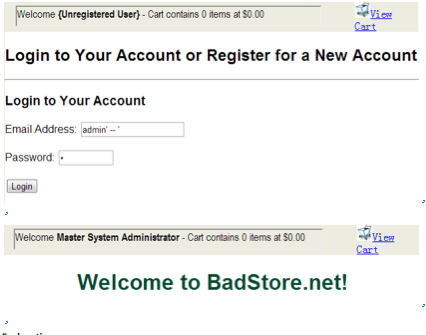
\includegraphics[height=2.5in]{sqli1}
  \end{center}
  \textbf{Explanation} Without injection, the SQL code is believed to be \lstinline{SELECT * FROM user WHERE EmailAddress = 'emailaddress' AND Password = 'password'}. Then during the injection, we input \lstinline{admin '--'} in the text box for the email address and some arbitrary password in the text box for the password. The WHERE condition is altered into \lstinline{WHERE EmailAddress = 'admin' -- ' AND Password = 'password'}, where the part following the two dashes is interpreted as a SQL comment. In other words, the WHERE condition is turned into \lstinline{WHERE EmailAddress = 'admin'}. Thus there is no need for a password and we can directly log into the admin account.
\item The result is shown below (Continued on next page):
  \begin{center}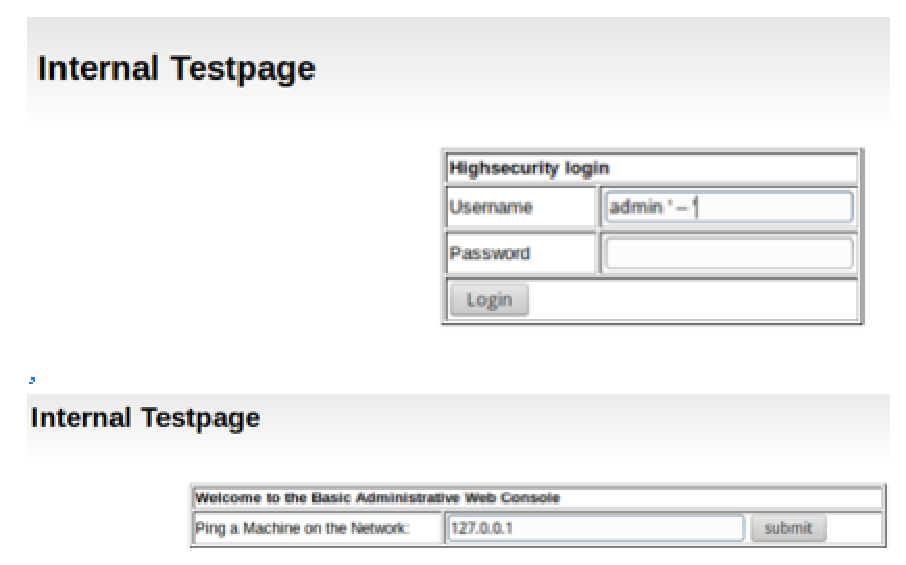
\includegraphics[height=2.5in]{sqli2}
  \end{center}
  \textbf{Explanation} The underlying SQL code for the login screen for host \ip{192.168.2.134} is believed to be the same as before: without injection, the SQL code is thought to be \lstinline{SELECT * FROM user WHERE UserName = 'username' AND Password = 'password'}. Then during the injection, we input \lstinline{admin '--'} in the text box for the username and some arbitrary password in the text box for the password. The WHERE condition is altered into \lstinline{WHERE UserName = 'admin' -- ' AND Password = 'password'} (or equivalently, \lstinline{WHERE UserName = 'admin'}). So there is no need for a password and we can directly log into the admin account.
\item \textbf{Prepared Statement} 
  A prepared statement, which is also called a parametrized statement, is a SQL query with variables inside of it. That is to say, we prepare the query with blank spots to fill and it will automatically protect the query from SQL injection.

  Here is a code snippet for using a prepared statement in PHP\cite{php}:
  \begin{lstlisting}[language = php]
    stmt = dbh->prepare("INSERT INTO REGISTRY (name, value) VALUES (:name, :value)");
    stmt->bindParam(':name', name);
    stmt->bindParam(':value', value);
  \end{lstlisting}

  In our case, we can create a prepared statement as follows:
  \begin{lstlisting}
    prepare("SELECT * FROM user WHERE UserName = :username AND Password = :password");
    bind(':username', username);
    bind(':password', password);
  \end{lstlisting}
  
  \textbf{Explanation}
  There are two variables in the prepared statement: username and password. Without injection, for instance with the username \lstinline{admin} and the password \lstinline{test}, the SQL query for logging on would be \lstinline{SELECT * FROM user WHERE username = 'admin' AND password = 'test'}. During an injection attempt, for instance with the username \lstinline{admin' --} and password \lstinline{123}, the SQL query becomes \lstinline{SELECT * FROM user WHERE username = 'admin\' --' AND password = '123'}. This is because the binding system will automatically change the input to protect the query. Thus, the SQL injection doesn't work in this situation.
\item The school lost all the student records because the table Students in the database is dropped by SQL injection. The SQL statement intended to be executed can be assumed to be of the form \lstinline{INSERT INTO Students VALUES ('Robert')}. The SQL injection had this query altered into the following two statements: \lstinline{INSERT INTO Students VALUES ('Robert'); DROP TABLE Students; --}. When the query is executed, the table Students will be dropped.

  What the school should do is to sanitize the database inputs by utilizing prepared statement as mentioned above. They can create prepared statement as follows:
  \begin{lstlisting}
    prepare("INSERT INTO Students VALUES (':name')");
    bind(':name',name);
  \end{lstlisting}

\end{enumerate}

\section*{Task 2: XSS and CSRF}
\subsection*{Exercises:}
\begin{enumerate}
\item The steps are as follows: 
	\begin{itemize}
		\item Open BadStore in your browser.
		\item Click "Sign Our GuestBook" on the left side of the page.
		\item In the "Your Name" field, type whatever you want.
		\item In the "Email" field, type whatever you want.
		\item In the "Comments" field, type \textit{<script>alert("1")</script>} .
		\item Click "Add Entry", the page should like this below:
		\par
		\begin{center}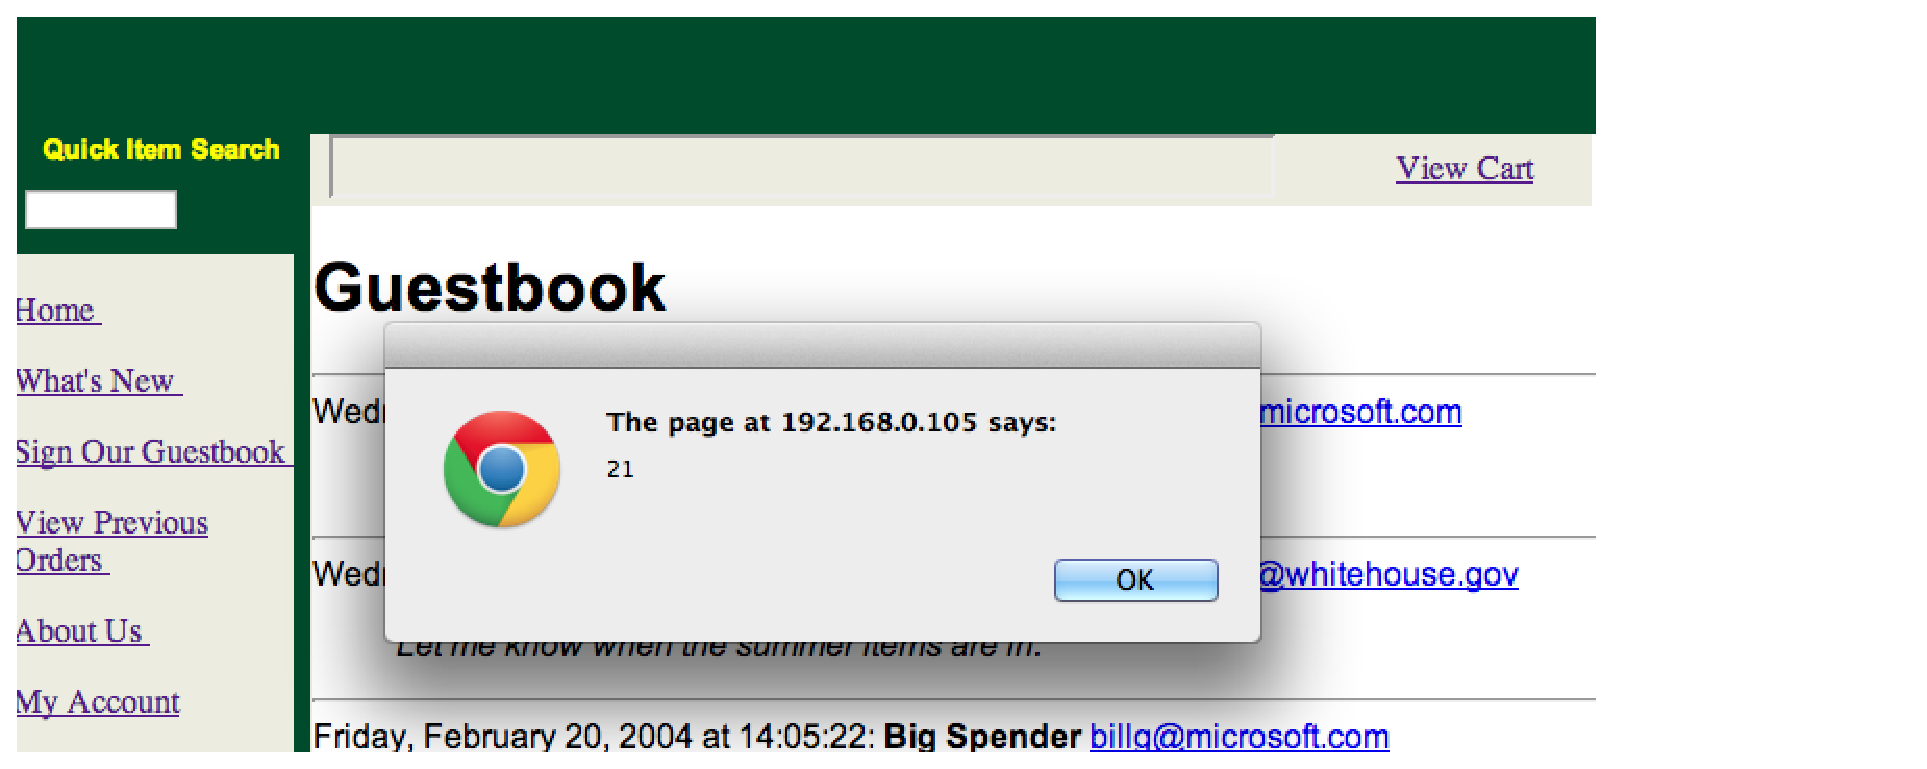
\includegraphics[height=2.5in]{xss}
		\end{center}
	\end{itemize}
	\indent Explanation: In the example, we write a piece of Javascript code in the comment area and submit it. It can work because the website has XSS vulnerability which enable us to insert and perform Javascript in the website. When it reloads, it will generate the current HTML code which contains the code we just injected. And it works as a result.
	\item To perform CSRF attacks, we need to create a custom web page contains deceived information. The function is to let user comment in the guestbook and receive countless alert. The key point is to guide victim to visit your page and click on the information. As the reason that we demonstrate it just as an example, we can suppose that the victim will click it. The custom page is so simple that it is just written as a demo. Below are the steps:
	\begin{itemize}
		\item Write a simple page containing these code:
		\par
		\begin{lstlisting}[language=HTML,numbers=left,numberstyle=\tiny,columns=fullflexible,basicstyle=\footnotesize\ttfamily]
<!DOCTYPE html>
<html>
<head>
	<title>iPhone Free!</title>
</head>
<body>
	<FORM METHOD="POST" ACTION="http://10.0.2.5/cgi-bin/badstore.cgi?action=doguestbook">
		<INPUT TYPE=hidden NAME=name value="<script>for(var i=0;i<10000;i++){alert('HHHH');}</script>" SIZE=30>
		<INPUT TYPE=hidden NAME=email value="1" SIZE=40>
		<TEXTAREA style="display:none" NAME=comments COLS=60 ROWS=4 value="aaa"> </TEXTAREA>
		<INPUT TYPE=submit VALUE="Get Now!">  
		<INPUT style="display:none" TYPE=reset></Center>
	</FORM>
</body>
</html>

		\end{lstlisting}
	\item The page shows like this:
	\begin{center}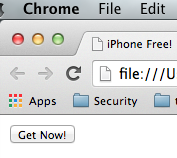
\includegraphics[height=2.5in]{csrf1}
	\end{center}
	\item Open BadStore and login in as an user.
	\item Click the "Get Now!" button in the custom page.
	\item The page will be redirected into BadStore and shows like this:
	\begin{center}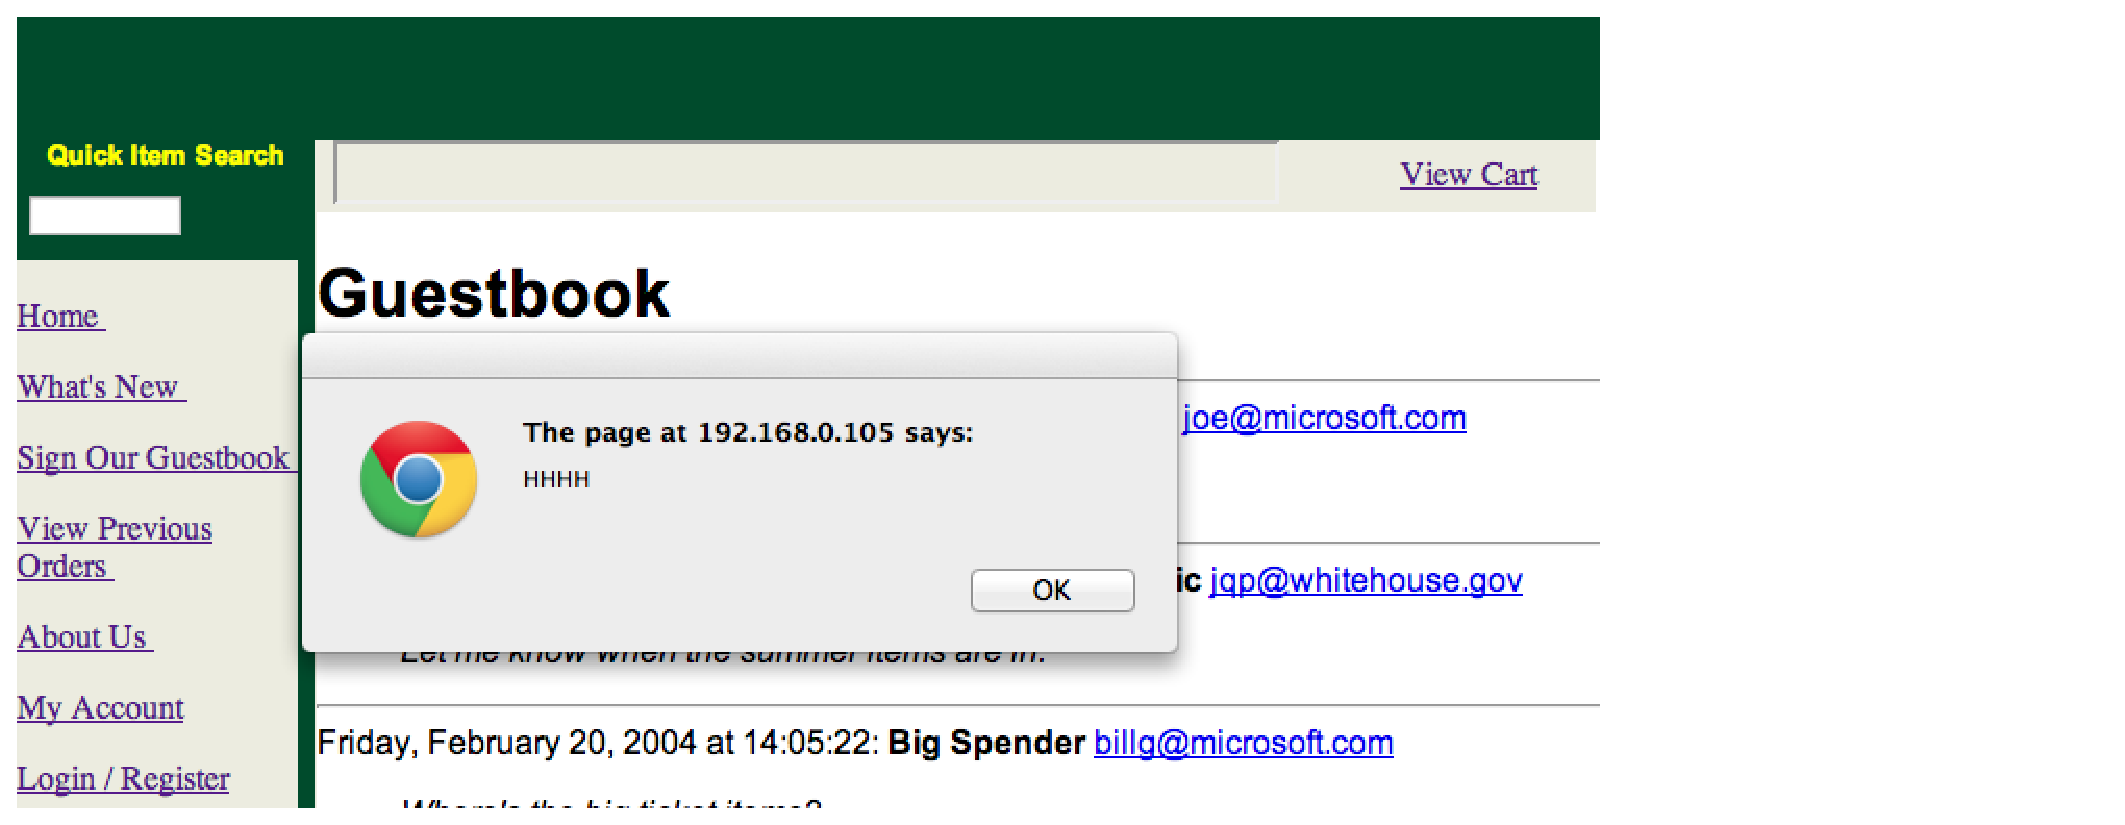
\includegraphics[height=2.5in]{csrf2}
	\end{center}
	\item The alert will repeat again and again as well as leaving many comments.
	\item Note: There might be some different performance in different browsers. i.e. Safari will operate the code after you quit it and reopen it.
	\end{itemize}
	\indent Explanation: In the example, we use a self-written page to perform CSRF attack. As mentioned above, the key point is that the attacker need to persuade the victim to visit the deceived page which contains evil code. The code can work with following reasons. First, the code will perform action in the server (BadStore) such as submitting an order or transferring money to another account. Second, the code will work because the victim doesn't close the server website. To make it clear, the cookie of the server website still exists in the browser. As a result, when the server receives the deceived request, it will think that the request is made by the victim and perform related operation.
	\item The difference is that, in an XSS attack, attacker makes the attack by inserting the  Javascript code inside the site. Because the site do not have strict check on user inputs, the code can be planted into HTML which will be operated on loading. On the contrary, CSRF attack don't necessarily need Javascript \cite{website:wikipedia_CSRF_XSS}. What counts most is that attacker must acquire trust from user and let him to operate the deceived request. Also, the user can't quit the page because the code will only work when the cookie of the target page stays. It's not the attacker himself that make it work.

\item \highergradesonly
\item \highergradesonly
\end{enumerate}

\section*{Task 3: Authentication}
The third and last task of the lab was about authentication, and the exercises were of a theoretical rather than practical nature.
\subsection*{Exercises:}
\begin{enumerate}
\item % (a)
Hashing a list of passwords with a one-way hash function, say $f$, rather than having the passwords stored in cleartext is a method for reducing the impact of a database leak. Authentication given a password $p$ in such a system is done by computing the hash $f(p)$ of the password and comparing it with the hash for the specific user stored in the database.

In the event that the password hashes are exposed to an attacker, there is no trivial way for him or her to retrieve the passwords corresponding to the compromised password hashes, by the definition of a one-way hash function. Thus, there is no trivial way of authenticating despite having access to both the hash function and the hashes. If an attacker finds the passwords stored in cleartext, on the other hand, he or she can authenticate as any of the affected users on the system. Furthermore, because passwords are frequently reused in more than one system, the attacker might be able to authenticate falsely on other systems as well. In other words, the impact of a cleartext password leak could encompass more than just the attacked system.

While there is no \emph{trivial} way of finding a password corresponding to a specific hash value, there is a cumbersome but in practice feasible way of doing so: password guessing. The idea is to repeatedly come up with a guess for the password, hash it, and compare the result with the hash value in question, continuing until a password guess with the specific hash is found. The hash values for guesses for common passwords can be precomputed into a so-called rainbow table that allow for these passwords to be looked up given their hash value.

Salting is a method for making password guessing more difficult. In addition to storing a hash value for each user, a random string $s$---the salt---is stored for each user as well. Authentication given a password $p$ is done by computing the hash of a combination of the password and the salt, such as $s + p$ where ``$+$'' denotes a concatenation. The resulting hash, $f(s + p)$, is then compared with the hash value in the database.

If an attacker gets hold of the database, which contains a salt and hash for each user, and aims for finding the password of \emph{any} of the users, the addition of the salt will make password guessing more difficult. Let $n$ be the number of users. Under the assumption that each user has a unique salt, the attacker will have to compute $n$ hashes for each password guess, compared to the single computation that is required with hashing alone. Salting offers increased security also against attacks with precomputed tables, seeing as one table would be needed for each possible salt in order to cover the same passwords as without salting.
\item % (b)
Assuming that the salt and salted hash are known to an attacker, salting may make the attack on a specific account more difficult, depending on whether precomputed tables are used.

If precomputed tables are used and the attacker did not choose the specific user because the attacker had a precomputed table for that specific salt, salting will make the attack more difficult in that more precomputed tables will be required.

Without precomputation, however, each password guess will require one computation of a hash value, assuming that the hash is computed like mentioned before: $f(s + g)$ for hash function $f$, salt $s$, password guess $g$, and concatenation operator $+$. The only difference in the case that salting is not used is that no salt has to be concatenated; the hash function still has to be evaluated once for each guess. Under the assumption that concatenating the string takes negligible time compared to evaluating the hash function, salting does not make the attack in question harder.
\item \highergradesonly
  \begin{itemize}
    \item
    \item
  \end{itemize}
\item % (d)
  \begin{itemize}
    \item
      While the fingerprint sensor of the iPhone 5s can evidently be deceived in a variety of ways, there are at least two reasons that it is a good addition to the iPhone security. The first reason is that the use of the fingerprint sensor in conjunction with more traditional authentication methods such as PIN codes adds another layer for the attacker to get past. The other reason, while not as convincing as the first, is that the sensor might provide a strong enough protection for some users, by the principle of adequate protection.
    \item
  \end{itemize}
\end{enumerate}

\end{document}
